\documentclass[11pt]{article}
\usepackage[a4paper,margin=23mm]{geometry}
\usepackage[T1]{fontenc}
\usepackage{lmodern,amsmath,amssymb,amsthm,mathtools,microtype,graphicx,booktabs}
\usepackage[colorlinks=true,linkcolor=blue,citecolor=blue,urlcolor=blue]{hyperref}
\newcommand{\HH}{\mathcal H}
\newcommand{\KK}{\mathcal K}
\newcommand{\Alg}{\mathcal A}
\newcommand{\DD}{\mathcal D}
\newcommand{\E}{\mathbb E}
\newcommand{\tr}{\operatorname{tr}}
\newcommand{\dd}{\mathrm d}
\newcommand{\norm}[1]{\left\lVert#1\right\rVert}
\newcommand{\sinc}{\operatorname{sinc}}
\newtheorem{proposition}{Proposition}
\title{The actual neutral slope in the selected Slater representation\\
\large Covariant amplification, selected densities and finite-resolution dephasing}
\author{Alan Day \and Chengheng\thanks{AI research assistant (OpenAI).}}
\date{8 November 2026\quad Local research draft}
\begin{document}\maketitle
\begin{abstract}
We connect the microscopic unpinched neutral-memory slope to the
same-disorder covariant size fluctuation in all fixed selected words.
The covariant subalgebra of the enlarged Slater representation is shown
to act as an amplification of the standard two-color $q$-Fock
representation. This identifies its compact quotient and gives an
explicit bounded density for one selected excitation. The density
controls finite-time energy averaging, whose trace variance decays as
$\kappa_u/T$. We obtain the ordered microscopic limit with double
scaling before removal of the averaging window. Exact finite-$N$
pinching is separately controlled in covariant words; its transfer to
selected excited words remains an explicit next problem.
\end{abstract}

\section{Actual operators and normalization}
Keep standard CAR, overlapping complex Hermitian Gaussian $p$-body
couplings $J$, even $N$, $m=N/2$ and the fixed occupied Slater set $O$.
Use the same $J$ for every operator. Set
\begin{equation}
 C_m=\E\tr_m H_N^2=w_N D_N,\quad
 D_N=\binom mp\binom{m+p}p,\quad L_N=\binom mp^2,
 \quad h_N=H_N/\sqrt{C_m}.
\end{equation}
The normalized selected creation block $M_N^\dagger$ is the sum of
the $O\to O^c$ disjoint $p$-hops with coefficient $J/\sqrt{L_N}$.
The state is $\varphi_N=\E\langle O|\,\cdot\,|O\rangle$.
Take $\lambda_N=p^2/N\to\lambda>0$, $q_N=e^{-4\lambda_N}\to q$,
$\gamma=q^{1/4}$ and $s=\sqrt q$. Averaging times below are
dimensionless, conjugate to $h_N$; physical string energies tend to
$(J_s/\sqrt\lambda)h$. The physical neutral slope has dimension
energy cubed.

The previous stage constructed
$u_N=(p-\mathcal L-\lambda_N)h_N/\sqrt{\lambda_N}$,
where $\mathcal L$ is full-Fock half-Clifford-size before charge
restriction. All selected mixed words and compact-time correlations
have a common positive limit $h,u,M$.
The present task is to connect an actual bilocal coefficient to this
representation. Established EGUE covariance \cite{Kota} and the
standard $q$-Fock representation \cite{Ricard} are inputs, not new
general covariance or Fock theorems.

\newpage
\section{Exact rank symbol and regression of the neutral slope}
Define the deterministic sandwich map using an independent Hamiltonian
only for the covariance average:
\begin{equation}
 \Phi_m(X)=\E_{H'}[H'_m XH'_m],\qquad
 \Phi_m/C_m=\mu_N(\mathcal R),
 \quad
 \mu_N(r)=\frac{\binom{m-r}p\binom{N-m+p-r}p}{D_N}.
\end{equation}
Here $\mathcal R$ labels the irreducible operator rank, not matrix
rank or particle-hole hop count. The normalized rank weights of $H$
are the existing EGUE weights
\begin{equation}\label{eq:weights}
 \omega_N(r)=
 \frac{[\binom Nr^2-\binom N{r-1}^2]
       \binom{m-r}{m-p}\binom{N-p-r}{m-p}}
      {\binom Nm D_N},\qquad 0\le r\le p.
\end{equation}
They sum to one. Put $\bar\mu_N=\sum_r\omega_N(r)\mu_N(r)$,
$\bar\kappa_m=C_m\bar\mu_N$, $\alpha=1-p/m$, $\epsilon=1-\alpha^2$.
The exact unpinched coefficient and its normalized version are
\begin{align}
 T_N&=m\epsilon\alpha[\Phi_m(H_N)-\bar\kappa_mH_N],\\
 t_N&=\frac{T_N}{8\lambda_N C_m^{3/2}q_N\sqrt{\lambda_N}}
      =f_N(\mathcal R)h_N,\label{eq:t}\\
 f_N(r)&=\frac{m\epsilon\alpha}{8\lambda_Nq_N\sqrt{\lambda_N}}
                   [\mu_N(r)-\bar\mu_N].
\end{align}
The actual exact-pinched slope is $B_{1,N}=(1-\mathcal P_{H_N})T_N$,
where $\mathcal P_{H_N}$ retains whole degenerate energy blocks.
Subtracting $\bar\kappa_m H_N$ before pinching changes nothing after
pinching; it fixes the useful unpinched regression.

Let $d=p-r$. The adjacent deficit probability ratio in
\eqref{eq:weights} is exactly
\begin{equation}
 \frac{\omega_N(r-1)}{\omega_N(r)}=
 \frac{a^2(1-b^2)}{1-a^2}
 \frac{m-r+1}{d+1}\frac{N-p-r+1}{N-m-r+1},\quad
 a=\frac r{N-r+1},\quad b=\frac{r-1}{N-r+2}.
\end{equation}
For fixed $d$ this tends to $\lambda/(d+1)$. For $p\le N/8$ and
$\lambda_N\le\lambda_+$ it is at most $8\lambda_+/(d+1)$.
Thus the full distribution is dominated by a constant times
$(8\lambda_+)^d/d!$, including every fixed polynomial weight. It
converges to Poisson$(\lambda)$ with all moments. This differs from
the Poisson$(2\lambda)$ deficit in the number of particles moved
by $H|O\rangle$; the two labels measure different things.

\newpage
\section{A microscopic bridge in every fixed selected word}
The exact product for $\mu_N$ gives, at fixed $d$,
\begin{equation}
 p[\mu_N(p-d)-\mu_N(p)]\longrightarrow4\lambda qd.
\end{equation}
For example, differentiate the logarithm along the bounded interval
$[p-d,p]$ and use $p/N\to0$. On the full deficit range the product
difference, estimated one factor at a time, gives
\begin{equation}
 0\le p[\mu_N(p-d)-\mu_N(p)]\le6\lambda_N d,
 \qquad p\le N/8.
\end{equation}
Indeed the sum of inverse denominators is at most
$p/(m-p)+p/(N-m)\le(14/3)p/N<6p/N$.
The other product factors lie in $[0,1]$.

Since $m\epsilon\alpha/p\to2$, the probability domination and
exact centering by $\bar\mu_N$ imply
\begin{equation}\label{eq:bridge}
 e_N^2:=\sum_{r=0}^p\omega_N(r)
 \left|f_N(r)-\frac{p-r-\lambda_N}{\sqrt{\lambda_N}}\right|^2
 \longrightarrow0.
\end{equation}
This is a dominated-convergence conclusion for the full rank sum,
not a rank cutoff or a fit to finite systems.

The difference of the two fields in \eqref{eq:bridge} is Hermitian,
linear Gaussian and $U(N)$-equivariant. Irreducibility on
$\bigwedge^m\mathbb C^N$ gives a scalar covariance $e_N^2 I_m$.
In real Gaussian coordinates its row and column coefficient norms
are consequently $e_N$. The preceding selected-word Wick contraction
bound supplies an $e_N$ factor for each telescoped error insertion;
the other fixed insertions have uniformly bounded coefficient norms.
The factorial tail extends this replacement to actual exponentials
of $h_N$ on compact complex-time windows. Finally the previous
central rank/size estimate
$\norm{(\mathcal R-\mathcal L)h_N}_{2,m}=O(N^{-1})$
has the same linear Gaussian covariance property. Combining the two
steps proves that $t_N$ and $u_N$ have the same fixed selected mixed
word and time limits.

There is a particularly direct finite-$N$ mixed check. A selected
disjoint $p$-hop is a pure rank-$p$ tensor; self-adjointness of the
rank multiplier therefore gives
\begin{equation}\label{eq:mixed}
 \varphi_N(t_N M_N^\dagger)
   =\sqrt{L_N/D_N}\,f_N(p)
   \longrightarrow-\sqrt\lambda\gamma.
\end{equation}
Equation \eqref{eq:mixed} tests the actual slope normalization and
its selected orientation, in addition to its tracial variance.
At the same time $\varphi_N(h_Nt_N)=0$ exactly by regression.

\newpage
\section{The entire covariant representation is a Fock amplification}
Use the preceding positive $H/U/P$ transfer, with orthogonal finite
grades $\HH_n$ and ordinary annihilators $a_H,a_U$. They obey
\begin{equation}
 a_i a_j^\dagger-q a_j^\dagger a_i=\delta_{ij}I,
 \qquad i,j\in\{H,U\}.
\end{equation}
Define $\mathcal V_n=\HH_n\cap\ker a_H\cap\ker a_U$.
It is the orthogonal complement in $\HH_n$ of the sum of the
two creation ranges from level $n-1$.

For $\xi,\eta$ in common-primitive spaces, normal order an inner
product between ordinary creation words applied to $\xi,\eta$.
Every uncontracted annihilator kills its primitive. If the primitive
grades differ, equal total grade still leaves an unmatched creator
or annihilator and the inner product is zero. If the grades agree,
the fully contracted terms are exactly the standard two-color
$q$-Fock Gram multiplied by $\langle\xi,\eta\rangle$.
Different total grades were already orthogonal. Positivity of the
ordinary $q$-Fock Gram and induction on the grade now give the
complete orthogonal decomposition
\begin{equation}\label{eq:amp}
 \HH\simeq\mathcal F_q(\mathbb R^2)\otimes\mathcal V,
 \quad \mathcal V=\bigoplus_{n\ge0}\mathcal V_n,
 \quad h=s_H\otimes I,\quad u=s_U\otimes I.
\end{equation}
Completeness follows because any complement at the next grade is
precisely $\mathcal V_n$. No formula for its multiplicities, and no
assumption that $\dim\HH_n=3^n$, is needed.

Let $C_q^*(\mathbb R^2)=C^*(1,s_H,s_U)$ in standard $q$-Fock space.
Equation \eqref{eq:amp} identifies $\DD=C^*(1,h,u)$ faithfully with
this algebra, and $\DD''$ with the amplified finite factor
$\Gamma_q(\mathbb R^2)\otimes I$. It contains no nonzero compact
operator. Otherwise a nonzero finite-rank spectral projection in
this factor would give a faithful finite-dimensional representation
of a diffuse corner, which is impossible.

The preceding stage proved $\Alg_+=\DD+\KK(\HH)$. The new
amplification therefore supplies the formerly missing injectivity
of the quotient restriction:
\begin{equation}
 \Alg_+/\KK(\HH)\simeq C_q^*(\mathbb R^2).
\end{equation}
This strengthens the earlier identification of only the
distinguished stationary state's GNS algebra. It does not by itself
classify every stationary state on the quotient.

\newpage
\section{An explicit density for a selected excitation}
Set $c=-\sqrt\lambda\gamma$ and $v=\gamma h+cu$.
The common primitive
\begin{equation}
 \zeta=M^\dagger\Omega-v\Omega,\qquad
 a_H\zeta=a_U\zeta=0,\qquad
 r_P:=\norm{\zeta}^2=1-s(1+\lambda)>0
\end{equation}
is orthogonal to the entire ordinary vacuum Fock copy.
Here $e^{2\lambda}>1+\lambda$ proves positivity. By
\eqref{eq:amp}, the two components evolve in orthogonal reducing
copies of the same ordinary field representation. For every
$B\in\DD$, and by normal extension for $B\in\DD''$,
\begin{equation}\label{eq:density}
 \varphi(M B M^\dagger)=\tau(\rho_1 B),\qquad
 \rho_1=v^2+r_PI,\qquad \tau(\rho_1)=1.
\end{equation}
The trace $\tau$ here is the standard two-color $q$-Gaussian trace.
It is the restriction of the preceding stationary state to $\DD$.
Since $v$ is an ordinary $q$-Gaussian field of variance
$s(1+\lambda)$,
\begin{equation}\label{eq:densitybound}
 r_PI\le\rho_1\le R_q I,\qquad
 R_q=\norm{\rho_1}=r_P+\frac{4s(1+\lambda)}{1-q}.
\end{equation}
For example \eqref{eq:density} gives
$\varphi(Mu^2M^\dagger)=1+\lambda s(1+q)$, independently recovering
the earlier four-point expression.

More generally any vector $\psi$ of finite grade can be written
under \eqref{eq:amp} as a finite sum
$\sum_j P_j(s_H,s_U)\Omega\otimes\kappa_j$, where the
$\kappa_j$ are orthonormal and $P_j$ are finite Wick polynomials.
The standard finite-tensor Wick representation is recalled in
\cite{Ricard}. Tracial cyclicity yields
\begin{equation}
 \langle\psi,B\psi\rangle=\tau(\rho_\psi B),\qquad
 \rho_\psi=\sum_j P_jP_j^\dagger\ge0.
\end{equation}
These densities are bounded. For general vectors they remain
normal $L^1$ densities, with no general boundedness assertion.

The residual $r_P$ measures the part of $M^\dagger\Omega$ outside
the full $h,u$ vacuum copy. It is different from the previous
$r_u=1-\lambda/(e^{2\lambda}-1)$, which measured the part of
$u\Omega$ outside the $h,M$ cyclic space. In particular
$r_P\to0$ whereas $r_u\to1/2$ as $\lambda\downarrow0$.
Neither formula is an interchange of the microscopic limits.

\newpage
\section{Finite-resolution dephasing in every selected vector}
For $T>0$ define the symmetric average in dimensionless time,
\begin{equation}
 D_T(X)=\frac1{2T}\int_{-T}^T e^{ith}Xe^{-ith}\,\dd t.
\end{equation}
Let $\rho_q(E)\dd E=\dd\mu_q(E)$ and $K_q(E,E')$ be the
standard $q$-Hermite measure and $q$-Mehler kernel of the preceding
stage. With $\sinc x=\sin x/x$, the two-energy formula gives
\begin{align}
 V_q(T):=\tau[(D_Tu)^2]
 &=\iint\sinc^2[T(E-E')]K_q(E,E')\,\dd\mu_q(E)\dd\mu_q(E'),\\
 &=\frac1T\int_0^{2T}\left(1-\frac t{2T}\right)C_u(t)\,\dd t.
\end{align}
At fixed $0<q<1$, the kernel is bounded and continuous on the
compact energy square. The density has square-root edges. Thus
the difference-energy density
$F(\omega)=\int K_q(E,E+\omega)\rho_q(E)\rho_q(E+\omega)\dd E$
is continuous at zero and compactly supported. The normalized
approximate identity $T\sinc^2(T\omega)/\pi$ proves
\begin{equation}\label{eq:asymptotic}
 T V_q(T)\longrightarrow\kappa_u
   =\pi\int K_q(E,E)\rho_q(E)^2\,\dd E>0.
\end{equation}
This is an ordinary Fourier consequence of the existing kernel.

Equations \eqref{eq:density}--\eqref{eq:densitybound} now turn it
into selected-state control:
\begin{equation}
 \norm{D_Tu\,M^\dagger\Omega}^2\le R_q V_q(T),\qquad
 \norm{D_Tu\,\psi}^2\le\norm{\rho_\psi}V_q(T)
\end{equation}
for every finite-grade $\psi$. These vectors are dense and
$\norm{D_Tu}\le\norm u$, so $D_Tu\to0$ strongly on the entire
enlarged Slater Hilbert space.

Use the same averaging window with the actual finite-$N$ $h_N$ and
set $b_{N,T}=(1-D_{N,T})t_N$. The regression term proportional to
$H_N$ cancels exactly, so this is the finite-resolution version
of the normalized actual slope. For fixed $T$, compact-time
convergence proves its joint limit $u-D_Tu$. Strong convergence
and uniform boundedness in the limiting representation then yield,
for every fixed selected word $W$,
\begin{equation}\label{eq:ordered}
 \lim_{T\to\infty}\lim_{N\to\infty}
 \varphi_N W(h_N,M_N,b_{N,T})=\varphi W(h,M,u).
\end{equation}
Adjoints and fixed external real-time insertions are allowed. This
is a microscopic ordered-limit statement; exact finite-$N$ pinching
uses the opposite order and requires a separate argument.

\newpage
\section{What exact pinching already permits, and what remains}
For covariant words alone, one can control exact pinching directly.
The central-sector positive two-energy measure $\nu_N$ defined by
$t_N$ converges weakly to $K_q\mu_q\otimes\mu_q$.
Fixed-word convergence supplies the moments and uniform high energy
moments give tightness; equivalently compact-time convergence gives
the characteristic functions. The limit has zero diagonal mass.
Portmanteau for the closed diagonal therefore gives
\begin{equation}
 \norm{\mathcal P_{H_N}t_N}_{2,m}^2
    =\nu_N\{E=E'\}\longrightarrow0.
\end{equation}
There is no exchange of infinite time and double scaling here.
Scalar Gaussian covariance bounds all fixed high Schatten moments
of $t_N$. Pinching is contractive on these norms, and interpolation
gives $\norm{\mathcal P_{H_N}t_N}_{r,m}\to0$ at every fixed finite
$r$. Schur invariance and tracial H\"older then transfer the actual
exact-pinched slope in every fixed purely covariant word and its
compact real-time correlations.

For words containing selected $M_N$ excitations this last tracial
step is not available. The limiting bounded density
\eqref{eq:density} does not automatically control the
$N$-dependent discontinuous energy projector. A sufficient next
estimate, for a fixed selected polynomial $P_N$, would be
\begin{equation}\label{eq:next}
 \E\langle O|P_N^\dagger Y_NP_N|O\rangle
 \le C_P\bigl(\E\tr_m Y_N^r\bigr)^{1/r},\qquad
 Y_N=(\mathcal P_{H_N}t_N)^2,
\end{equation}
with $r$ fixed and $C_P$ independent of $N$. We have not proved
\eqref{eq:next}, nor asserted it for arbitrary covariant positive
$Y_N$. A direct bound exploiting this particular slope and its
energy projection could replace it.

The concrete next task is this selected exact-pinching interface,
then the quadratic field $J_2$ and complete bilocal in the common
representation. The older full-trace complete bilocal four-point
construction is already available. Spatial and mass generators,
the physical temperature assignment and finite-$G$ dynamics remain
separate required parts of the de Sitter program.

The representation change is consistent with the distinction
between generic and state-adapted observables emphasized in
\cite{RX}. The new contribution here is the explicit same-$J$
neutral-slope interface, amplification and selected density;
it is not a replacement of the original model by independent matter.

\newpage
\section{Sealed checks and numerical scale of dephasing}
\begin{center}
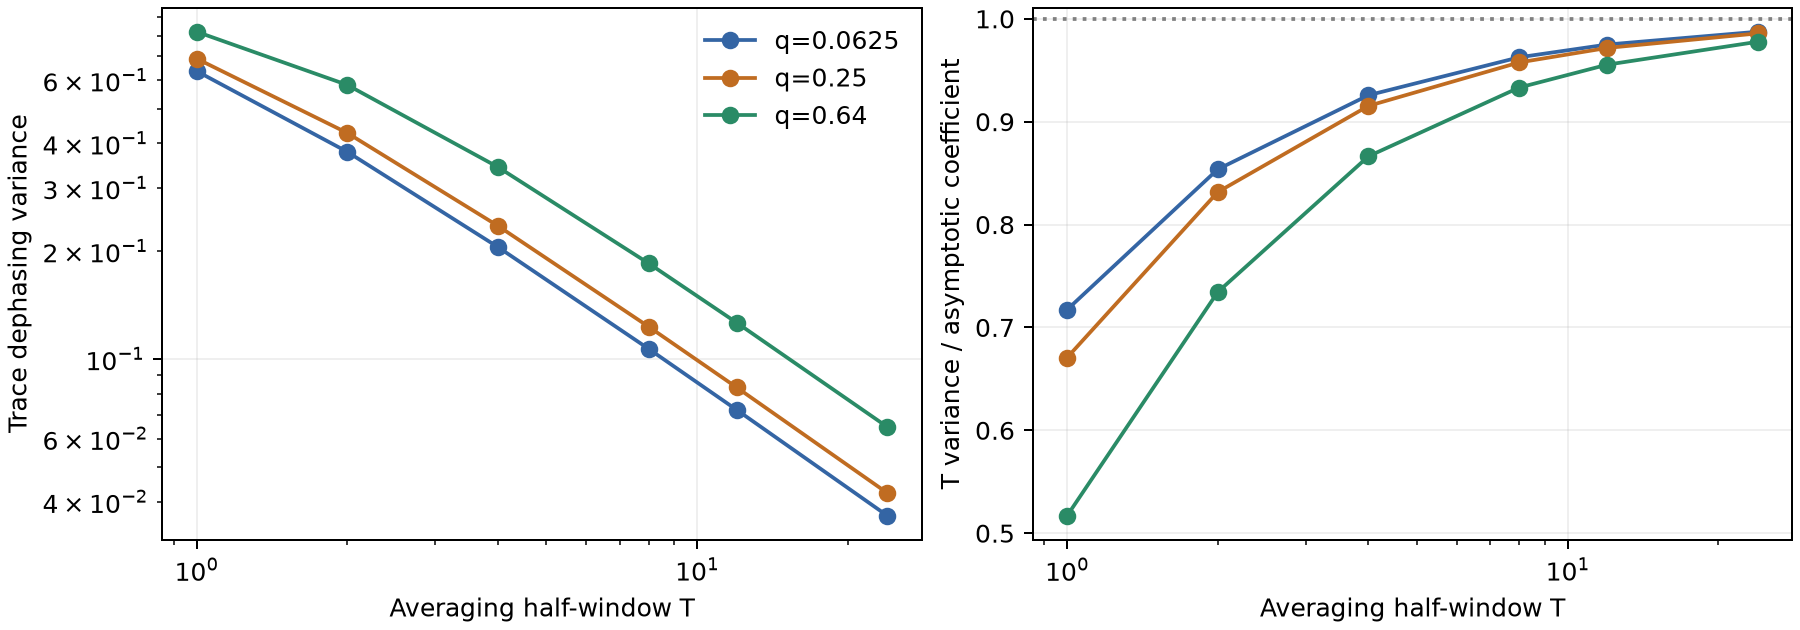
\includegraphics[width=\linewidth]{../../results/susskind-slater-neutral-slope/neutral-slope-dephasing.png}
\end{center}
The left panel shows $V_q(T)$; the right tests its asymptotic
coefficient in \eqref{eq:asymptotic}. At fixed Jacobi dimension $L$,
infinite time instead gives a positive diagonal plateau. This
plateau is recorded and is not interpreted as continuum zero-frequency
mass. The exact-arithmetic error of the finite-$L$ variance is at
most $4e^x x^L/L!$, $x=2TE_*$, $E_*=2/\sqrt{1-q}$, by integrating
the preceding banded-Taylor correlation bound. Roundoff is not
included in this analytic bound.

Three new successful outputs are sealed without rerunning earlier
scientific drivers. The rank output contains 20 exact rational
systems and 12 physical all-rank sums at 80 and 120 digits, with all
$p+1$ probabilities and slope coefficients retained. Finite deviations
from the limit are reported, not used as pass thresholds.
The amplification output checks 1022 density identities, eight
common-primitive vectors and 32 tower inner products exactly.
Its independent rational $\gamma,\sqrt\lambda$ parameters check
algebra, not the physical curve $q=e^{-4\lambda}$.

The dephasing output uses three physical $q$ values, $T=1,2,4,8,12,24$,
Jacobi dimensions 512 and 768 (36 rows), and two diagonal-density
quadratures. An independent triangular time integral differs by
$1.82\times10^{-13}$. These finite checks do not prove the
infinite-dimensional decomposition or the limit exchange.
Code, versions, parameters, scientific outputs, PDF build and page
renders are bound by the stage SHA256 manifest.

\begin{thebibliography}{9}\small
\bibitem{Kota} V. K. B. Kota,
\emph{SU(N) Wigner--Racah algebra for the matrix of second moments
of embedded Gaussian unitary ensemble of random matrices},
\href{https://arxiv.org/abs/nucl-th/0410069}{arXiv:nucl-th/0410069},
Secs.~III--IV.
\bibitem{Ricard} E. Ricard, \emph{Factoriality of $q$-Gaussian von Neumann algebras},
\href{https://arxiv.org/abs/math/0311413}{arXiv:math/0311413v2}, Sec.~2.
\bibitem{RX} H. Rajgadia and J. Xu,
\emph{Emergent States and Algebras from the Double-Scaling limit of Pure States in SYK},
\href{https://arxiv.org/abs/2604.14387}{arXiv:2604.14387v3}, Secs.~4.1--4.2.
\end{thebibliography}
\end{document}
